\documentclass{article}

\usepackage[]{graphicx}
\usepackage[]{amsmath}

\title{Why trade is good (and free trade is better)}

\begin{document}

\maketitle

Consider the following model. Two countries, England and Portugal, both produce the goods
\textbf{cloth} and \textbf{wine}. However, the labor involved in producing these goods differ by
product and across country lines. In particular, the number of hours required to produce one unit of
each of these goods is given in the table below:

\begin{center}
  \begin{tabular}[]{ccc}
    & Cloth & Wine \\
    England & 100 & 120 \\
    Portugal & 90 & 80
  \end{tabular}
\end{center}

So, for example, in this world it takes England 100 hours to produce one unit of cloth. It is clear
that Portugal is better at producing both cloth and wine than England is, because whereas it takes
England 100 hours to produce a unit of cloth, it only takes Portugal 90, and whereas it takes
England 120 hours to produce a unit of wine, it only takes Portugal 80. In economics jargon, this
means that Portugal has an \textbf{absolute advantage} in producing both cloth and wine. In the
world of international relations in which trade is illegal, both countries can only use their own
labor resources. For example, if both countries have 100 hours of labor to allocate, then the
production possibilities will be distributed according to the picture below:

\begin{center}
  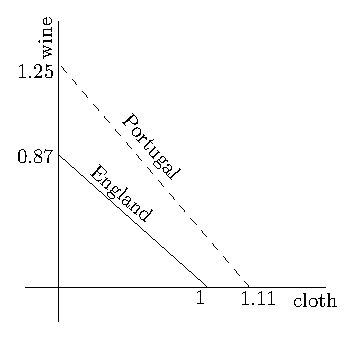
\includegraphics[width=0.5\textwidth]{../ipe-graphics/2018-11-21-comparative-advantage.eps}
\end{center}

This picture indicates that any possible production bundle for England lies on the filled line,
whereas any possible production bundle for Portugal lies on the dotted line.  Notice that even
though Portugal has an absolute advantage in producing cloth, England has a \textbf{comparative
advantage} in producing cloth. To see why, notice that the relative ``cost'' of producing cloth
instead of wine in England is 
\begin{equation*}
  100 / 120 = 0.87
\end{equation*}
whereas the relative cost of producing cloth instead of wine in Portugal is
\begin{equation*}
  90 / 80 = 1.125.
\end{equation*}
This means that it's ``cheaper'' for England to allocate more labor towards cloth-making than it is
for Portugal to do so. 

In the no-trade scenario, the best either country can do is hit their maximum production in 100
hours (that is, fall somewhere on their respective lines). However, in the free-trade scenario, both
countries can specialize to the products they have comparative advantages in. So England spends all
100 hours making cloth (totalling 1 unit) whereas Portugal spends all 100 hours making wine
(totalling 1.125 units). If the world market for cloth puts the price between 0.87 and 1.125 units
of wine, then English cloth may be traded for Portuguese wine so that both countries end up with a
production level that is \emph{strictly larger} than before. For example, say that one unit of cloth
is worth one unit of wine. If England trades 0.125 units of cloth for Portugal's 0.125 units of
wine, then the resulting bundle for England is $(0.875,0.125)$ and for Portugal is $(0.125, 1)$.
Both of these production levels are \emph{impossible without free-trade}. 

What about the trade deficit? The trade deficit of England is the difference between exports and
imports: $X - J$. On the other hand, the income of England is net exports plus consumption,
investment, and government spending:
\begin{equation*}
  Y = C + I + G + (X - J).
\end{equation*}
Consumption is income minus taxes and savings:
\begin{equation*}
  C = Y - T - S.
\end{equation*}
Hence
\begin{equation*}
  Y = Y - T - S + I + G + (X - J)
\end{equation*}
which implies
\begin{equation*}
  (S - I) = (G - T) + (X - J).  
\end{equation*}
This is an accounting identity. It must hold. Now assume that England has a trade deficit with
Portugal, so that $X - J < 0$. Then
\begin{equation*}
  (S-I) > (G-T).
\end{equation*}
England always runs a government fiscal deficit, which means that $G-T > 0$. So in the trade deficit
scenario, $S - I > 0$ means that England is saving more than it's investing. On the other hand,
suppose England has a trade surplus with Portugal. Then all of the reverse statements hold; i.e.,
England is investing more than it's saving.

Returning to the identity
\begin{equation*}
  (S - I) = (G - T) + (X - J),
\end{equation*}
now suppose that the fiscal deficit \emph{increases} (say, due to a reckless tax cut). Then because
this equation must balance, this implies that either domestic investment goes down or the trade
deficit must also increase. The fastest way for the government to lower the trade deficit, then, is
to raise taxes! 

On the other hand, one can show that in an open economy, the effect of a recession (from, say, a
decline in consumption) on GDP is less damaging under a regime of free trade than under a closed
system. What this means is that recessions hurt less with free trade.




\end{document}
